\chapter{Der Higgs-Mechanismus: Wie ein Eichboson Masse erhält}

Wir verbinden nun die beiden Ideen aus der vorherigen Vorlesung. Ein komplexes Skalarfeld mit gebrochener globaler \(U(1)\)-Symmetrie besitzt eine massive radiale Schwingung und eine masselose Winkelschwingung. Eine lokal invariante \(U(1)\)-Theorie enthält ein masseloses Eichfeld. Ist das Skalarfeld geladen und sein Gleichgewichtsbetrag ungleich null, lassen sich diese Aussagen nicht einfach zusammenfügen. Der Winkelmodus und das Eichfeld verbinden sich: Das Eichfeld wird massiv, das scheinbare Goldstone-Boson ist kein unabhängiges Teilchen mehr, und der radiale Higgs-Modus bleibt erhalten.

Das Photon dient uns als Modell-Eichboson, nicht aber als physikalische Schlussfolgerung. Die elektromagnetische \(U(1)\)-Symmetrie ist im Vakuum nicht gebrochen, daher ist das reale Photon masselos. Derselbe Mechanismus wirkt in der elektroschwachen Theorie auf das \(W^\pm\) und das \(Z\); dort sind die Eichgruppe und das Skalarmultiplett komplizierter. Das abelsche Modell macht den Mechanismus sichtbar, ohne ihn hinter Gruppentheorie zu verbergen.

\begin{classroomqa}
\audiencequestion{Bedeutete die vorherige Diskussion, dass der Higgs-Mechanismus dem realen Photon Masse verleiht?\lecturetimestamp{00:00:23}}
\lecturerresponse{Nein. Wir fragen, was geschehen würde, \emph{wenn} die mit dem Photon verbundene \(U(1)\)-Symmetrie gebrochen wäre. Dieses hypothetische Photon würde massiv. Das reale elektromagnetische Vakuum befindet sich nicht in dieser Phase; in der Teilchenphysik geht es stattdessen um die Masse des \(W\) und des \(Z\).}
\end{classroomqa}

Die mit der Erhaltung der elektrischen Ladung verbundene Symmetrie ist die Phasendrehung
\begin{equation}
  \phi(x)\longmapsto e^{i\theta}\phi(x),
\end{equation}
eine interne Drehung, die als \(U(1)\) bezeichnet wird. Ein Supraleiter bietet ein reales Analogon der gebrochenen Phase. In seinem Inneren hat das elektromagnetische Feld eine endliche Eindringtiefe und verhält sich in wichtigen Hinsichten wie ein massives Feld. Außerhalb tritt wieder das gewöhnliche masselose Photon auf.

\section{Was Masse für ein Feld bedeutet}

\subsection{Dispersion und die Lücke bei verschwindendem Impuls}

Bevor wir das Higgs-Feld einführen, sollten wir genau festlegen, was wir unter Masse verstehen. Für eine Welle gilt
\begin{equation}
  E=\hbar\omega,
  \qquad
  p=\hbar k,
  \label{eq:l08-quantum-wave}
\end{equation}
Ein \((E,p)\)-Diagramm und ein \((\omega,k)\)-Diagramm enthalten also bis auf Faktoren von \(\hbar\) dieselbe Information. Im leeren Raum erfüllt eine masselose relativistische Anregung
\begin{equation}
  E=c|p|,
  \qquad
  \omega=c|k|.
  \label{eq:l08-massless-dispersion}
\end{equation}
Die beiden Vorzeichen von \(k\) kennzeichnen entgegengesetzte Ausbreitungsrichtungen. Entscheidend ist, dass \(\omega\) mit \(k\) gegen null geht.

Für ein massives relativistisches Teilchen gilt
\begin{equation}
  E^2=c^2p^2+m^2c^4.
  \label{eq:l08-massive-dispersion}
\end{equation}
In Einheiten mit \(c=\hbar=1\) gilt
\begin{equation}
  \omega^2=k^2+m^2.
\end{equation}
Bei \(k=0\) beträgt die Energie \(E=mc^2\), oder in natürlichen Einheiten einfach \(m\). Masse ist somit die von null verschiedene Energielücke des Modus mit verschwindendem Impuls.

\begin{figure}[htbp]
\centering
\begin{adjustbox}{max width=\linewidth}
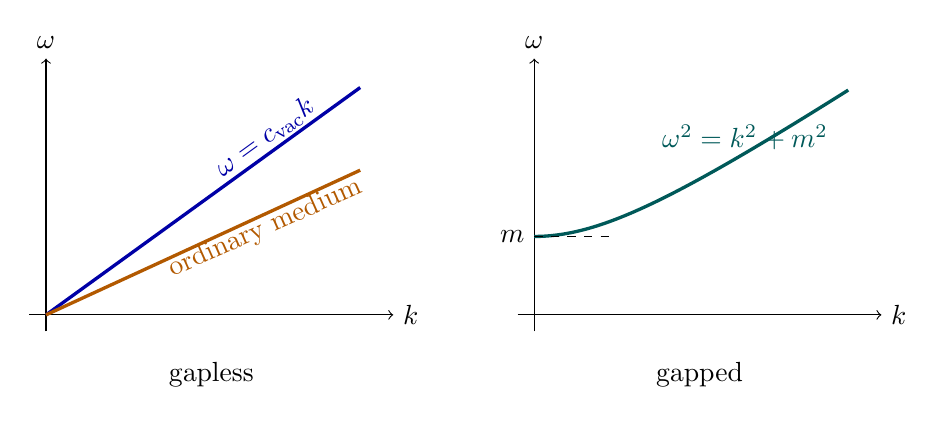
\begin{tikzpicture}[x=1.05cm,y=1.05cm]
  \begin{scope}
    \draw[->] (-0.2,0) -- (4.2,0) node[right] {\(k\)};
    \draw[->] (0,-0.2) -- (0,3.1) node[above] {\(\omega\)};
    \draw[very thick,blue!65!black] (0,0) -- (3.8,2.75);
    \draw[very thick,orange!70!black] (0,0) -- (3.8,1.75);
    \node[blue!65!black,rotate=36] at (2.65,2.15)
      {\(\omega=c_{\rm vac}k\)};
    \node[orange!70!black,rotate=24] at (2.65,1.05)
      {ordinary medium};
    \node[below] at (2,-0.45) {gapless};
  \end{scope}
  \begin{scope}[xshift=6.2cm]
    \draw[->] (-0.2,0) -- (4.2,0) node[right] {\(k\)};
    \draw[->] (0,-0.2) -- (0,3.1) node[above] {\(\omega\)};
    \draw[very thick,domain=0:3.8,samples=120,smooth,teal!70!black]
      plot (\x,{sqrt(0.9+0.45*\x*\x)});
    \draw[dashed] (0,0.95) -- (1.0,0.95);
    \node[left] at (0,0.95) {\(m\)};
    \node[teal!70!black] at (2.55,2.15)
      {\(\omega^2=k^2+m^2\)};
    \node[below] at (2,-0.45) {gapped};
  \end{scope}
\end{tikzpicture}
\end{adjustbox}
\caption{Eine Änderung der Ausbreitungsgeschwindigkeit ändert die Steigung einer lückenlosen Dispersionsrelation. Eine Masse der Anregung öffnet bei \(k=0\) eine endliche Lücke.}
\label{fig:l08-dispersion}
\end{figure}

Ein gewöhnliches transparentes Material kann die Phasengeschwindigkeit einer Welle herabsetzen, ohne diese relativistische Masselücke zu erzeugen. An einer Grenzfläche bleibt die Frequenz der einfallenden Welle fest, während sich die Wellenzahl an die Dispersionsrelation des Mediums anpasst. Die Steigung zu ändern ist nicht dasselbe, wie den Achsenabschnitt anzuheben.
\editorialnote{Ein Material kann mehrere elektromagnetische Zweige besitzen, und in einem Plasma oder einem resonanten Medium kann eine endliche Plasmafrequenzlücke auftreten. Der Vergleich in dieser Vorlesung betrifft ausdrücklich einen gewöhnlichen Brechungszweig und die Antwort eines Supraleiters. Allgemeiner bedeutet Lückenlosigkeit, dass \(\omega(k)\to0\) für \(k\to0\) gilt; exakte Linearität ist nicht in jedem nichtrelativistischen Medium erforderlich.}

\begin{classroomqa}
\audiencequestion{Erhält ein Photon immer dann Masse, wenn es sich durch Materie bewegt, zum Beispiel durch ein Prisma?\lecturetimestamp{00:03:02}}
\lecturerresponse{Nein. Die Brechung kann die Beziehung zwischen Frequenz und Wellenzahl und damit die Ausbreitungsgeschwindigkeit ändern, während der Zweig bei \(\omega=0\) weiterhin durch \(k=0\) verläuft. In einer supraleitenden Phase erhält die elektromagnetische Antwort dagegen eine endliche inverse Eindringlänge, das Analogon einer Masse.}
\end{classroomqa}

\begin{classroomqa}
\audiencequestion{Ändert sich die Wellenzahl, wenn Licht mit fester Frequenz in Glas eintritt?\lecturetimestamp{00:09:20}}
\lecturerresponse{Ja. Die Zeittranslationsinvarianz an einer stationären Grenzfläche hält die Frequenz konstant. Da die Dispersionskurve im Glas eine andere Steigung hat, entspricht dasselbe \(\omega\) einem anderen \(k\) und damit einer anderen Wellenlänge.}
\end{classroomqa}

Die Steigung
\begin{equation}
  v_g=\frac{d\omega}{dk}
\end{equation}
ist die Gruppengeschwindigkeit eines Wellenpakets. Ändert sich diese Steigung mit \(k\), bewegen sich verschiedene Fourier-Komponenten mit unterschiedlichen Geschwindigkeiten, und das Paket dispersiert. Deshalb heißt die Beziehung \(\omega(k)\) \emph{Dispersionsrelation}.

\begin{classroomqa}
\audiencequestion{Wie heißt die Kurve, und was bedeutet ihre Steigung?\lecturetimestamp{00:11:02}}
\lecturerresponse{Die Kurve ist die Dispersionsrelation. Ihre Ableitung \(d\omega/dk\) ist die Gruppengeschwindigkeit. Bei konstanter Steigung haben alle Wellenlängen dieselbe Geschwindigkeit; bei veränderlicher Steigung breitet sich ein Wellenpaket aus. Für unseren Zweck ist entscheidend, ob die Kurve den Ursprung erreicht oder eine Lücke aufweist.}
\end{classroomqa}

\subsection{Eine homogene Schwingung entspricht einem Teilchen in Ruhe}

Der Modus \(k=0\) hat eine unendliche Wellenlänge: Das Feld ist überall um denselben Betrag ausgelenkt. Gibt man eine homogene Auslenkung frei, so schwingt das Feld mit einer von null verschiedenen Frequenz, falls die zugehörige Quante eine von null verschiedene Ruheenergie besitzt und damit massiv ist. Fehlt in dieser Richtung eine rücktreibende Kraft, verschwindet die Frequenz und der Modus ist masselos.

Diese Aussage ist klassisch. Sie setzt nicht voraus, dass räumlich getrennte Teilchen sich in einer quantenmechanischen Superposition befinden. Eine homogene klassische Feldkonfiguration ist schlicht ein Feldwert, der im gesamten Raum denselben Wert hat.

\begin{classroomqa}
\audiencequestion{Wenn ein ganzes Feld gemeinsam verschoben wird, ist das dasselbe wie Quantenverschränkung?\lecturetimestamp{00:10:04}}
\lecturerresponse{Nein. Ein homogenes klassisches Feld ist eine einzige klassische Konfiguration. Verschränkung korreliert verschiedene Quantenalternativen, etwa die Spinkonfigurationen oben--unten und unten--oben. An vielen Orten denselben Feldwert einzustellen, ist für sich genommen keine Verschränkung und bedeutet auch keine augenblickliche kausale Reaktion.}
\end{classroomqa}

Für ein kanonisch normiertes reelles Feld gilt
\begin{equation}
  \mathcal L
  =\frac12\partial_\mu\varphi\,\partial^\mu\varphi-V(\varphi),
\end{equation}
Wir entwickeln um ein Gleichgewicht \(\varphi_0\):
\begin{equation}
  V(\varphi_0+\eta)
  =V(\varphi_0)
   +\frac12V''(\varphi_0)\eta^2+\cdots.
\end{equation}
Am Minimum verschwindet der lineare Term, und die Feldgleichung ergibt
\begin{equation}
  \omega^2=\bm{k}^2+m^2,
  \qquad
  m^2=V''(\varphi_0).
  \label{eq:l08-curvature-mass}
\end{equation}
Die Masse entspricht somit der Krümmung des Potentials in Bewegungsrichtung. Eine flache Richtung hat keine Krümmung und ergibt einen masselosen Modus.

\section{Das gebrochene komplexe Skalarfeld}

\subsection{Radiale und tangentiale Bewegung}

Wir schreiben ein komplexes Skalarfeld in kartesischen und Polarkoordinaten:
\begin{equation}
  \phi=\phi_R+i\phi_I=\rho e^{i\alpha},
  \qquad
  \phi^*=\phi_R-i\phi_I=\rho e^{-i\alpha}.
  \label{eq:l08-polar-field}
\end{equation}
Die komplexe Ebene ist ein \emph{interner} Feldraum. An jedem physikalischen Raumzeitpunkt \(x\) legt das Paar
\((\phi_R(x),\phi_I(x))\)einen Punkt in dieser internen Ebene fest.
Keine der beiden internen Achsen ist eine Richtung im Labor.

\begin{figure}[htbp]
\centering
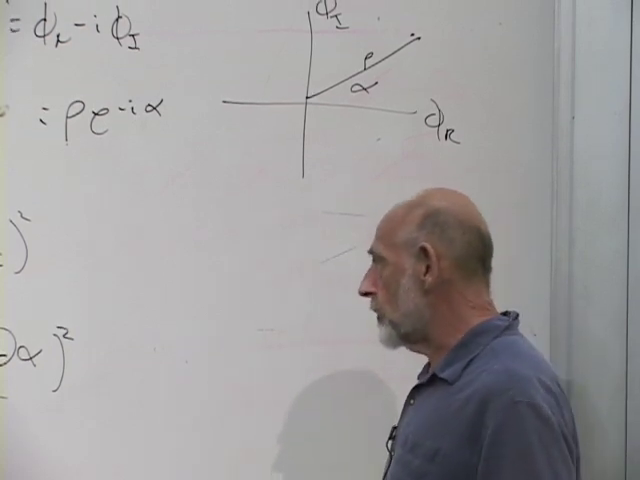
\includegraphics[width=0.72\textwidth]{lecture_08_figure_02.png}
\caption{Das komplexe Skalarfeld in seiner internen \((\phi_R,\phi_I)\)-Ebene. Der Radius ist \(\rho\), und \(\alpha\) bezeichnet die interne Phase.}
\lectureframe{00:24:41}
\label{fig:l08-internal-plane}
\end{figure}

Der kinetische Term des Skalarfelds wird zu
\begin{align}
  \partial_\mu\phi^*\,\partial^\mu\phi
  &=
  \partial_\mu\phi_R\,\partial^\mu\phi_R
  +\partial_\mu\phi_I\,\partial^\mu\phi_I
  \notag\\
  &=
  \partial_\mu\rho\,\partial^\mu\rho
  +\rho^2\partial_\mu\alpha\,\partial^\mu\alpha.
  \label{eq:l08-polar-kinetic}
\end{align}
Ein globales \(U(1)\)-invariantes Potential hängt von \(\phi^*\phi=\rho^2\) ab, nicht von \(\alpha\). Zum Beispiel:
\begin{equation}
  V(\phi)
  =\lambda\left(\phi^*\phi-\frac{f^2}{2}\right)^2,
  \qquad \lambda>0.
  \label{eq:l08-mexican-hat}
\end{equation}
Die Minima bilden einen Kreis. Das Gesetz ist unter einer gemeinsamen Phasendrehung invariant, doch die Wahl einer Gleichgewichtsphase zeichnet einen Punkt auf dem Kreis aus.

\begin{figure}[htbp]
\centering
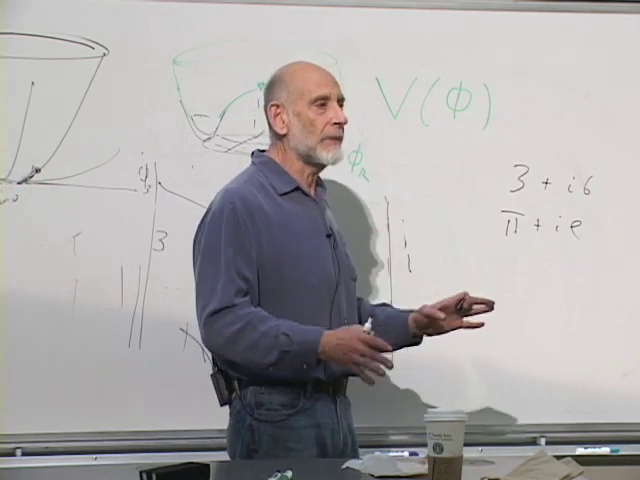
\includegraphics[width=0.78\textwidth]{lecture_08_figure_03.png}
\caption{Skizzen des radialen Potentials an der Tafel. Das Potential ist gegenüber Drehungen des internen Feldwerts symmetrisch, obwohl das Feld selbst nicht im Ursprung liegen muss.}
\lectureframe{00:34:22}
\label{fig:l08-radial-potential-board}
\end{figure}

\begin{figure}[htbp]
\centering
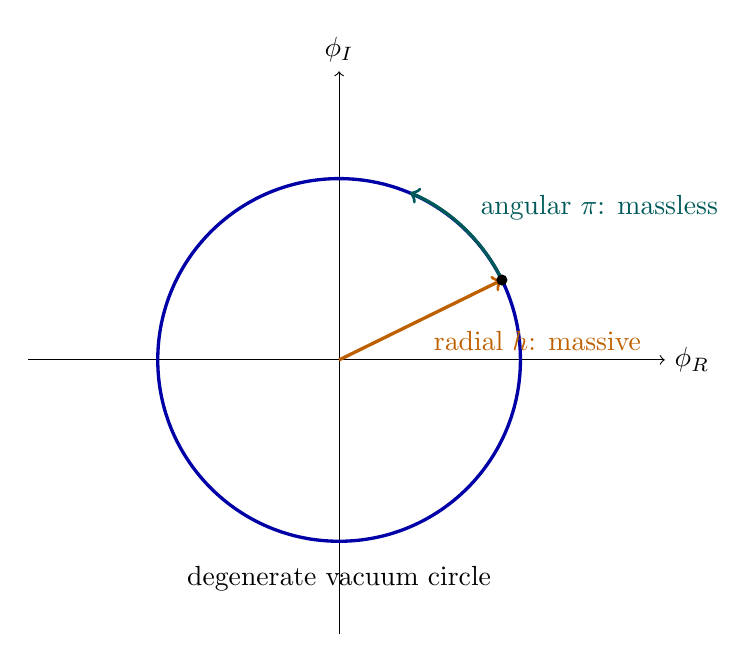
\begin{tikzpicture}[x=0.94cm,y=0.94cm]
  \draw[->] (-4.2,0) -- (4.4,0) node[right] {\(\phi_R\)};
  \draw[->] (0,-3.7) -- (0,3.9) node[above] {\(\phi_I\)};
  \draw[very thick,blue!65!black] (0,0) circle (2.45);
  \draw[->,very thick,orange!75!black] (0,0) -- (2.2,1.08);
  \draw[->,very thick,teal!70!black]
    (2.2,1.08) arc[start angle=26,end angle=67,radius=2.45];
  \node[orange!75!black,below right] at (1.15,0.52)
    {radial \(h\): massive};
  \node[teal!70!black,above right] at (1.78,1.76)
    {angular \(\pi\): massless};
  \fill (2.2,1.08) circle (2pt);
  \node[below] at (0,-2.65) {degenerate vacuum circle};
\end{tikzpicture}
\caption{Die global gebrochene Theorie besitzt eine Krümmung senkrecht zum Vakuumkreis, aber keine Krümmung entlang des Kreises. Der radiale Higgs-Modus ist massiv, der winkelabhängige Goldstone-Modus masselos.}
\label{fig:l08-radial-angular}
\end{figure}

Wir setzen
\begin{equation}
  \phi(x)=\frac{f+h(x)}{\sqrt2}
           e^{i\pi(x)/f}.
  \label{eq:l08-canonical-polar}
\end{equation}
In der Nähe des ausgewählten Vakuums beschreibt \(h\) die radiale Auslenkung und \(\pi\) die tangentiale Auslenkung, jeweils mit kanonischer Normierung. Einsetzen in Gl.~\eqref{eq:l08-polar-kinetic} ergibt
\begin{equation}
  \partial_\mu\phi^*\,\partial^\mu\phi
  =
  \frac12(\partial_\mu h)^2
  +\frac12\left(1+\frac{h}{f}\right)^2
            (\partial_\mu\pi)^2.
  \label{eq:l08-global-expanded}
\end{equation}
Das Potential aus Gl.~\eqref{eq:l08-mexican-hat} liefert
\begin{equation}
  m_h^2=2\lambda f^2,
  \qquad
  m_\pi^2=0.
  \label{eq:l08-global-masses}
\end{equation}
Bei Energien weit unterhalb von \(m_h\) ist eine radiale Bewegung energetisch aufwendig, daher können wir \(h=0\) vorübergehend festhalten. Die verbleibende Lagrange-Funktion enthält nur \(\frac12(\partial\pi)^2\), ohne einen Term \(\pi^2\). Dies ist das Goldstone-Boson.\editorialnote{An zwei Stellen kehrt die mündliche Erklärung die Bezeichnungen um und sagt, dass das Verschlucken des Goldstone-Bosons dem Higgs-Boson seine Masse verleihe. Die Rechnung an der Tafel und der Rest der Vorlesung belegen das beabsichtigte Ergebnis: Die radiale Krümmung verleiht dem Higgs-Modus bereits Masse, während das Eichboson den Goldstone-Modus aufnimmt und massiv wird.}

\begin{classroomqa}
\audiencequestion{Ist dies die einzige spontane Symmetriebrechung im Standardmodell?\lecturetimestamp{00:16:39}}
\lecturerresponse{Die elektroschwache Higgs-Phase ist der hier relevante, etablierte Mechanismus der Symmetriebrechung. Die tatsächliche Symmetrie ist \(SU(2)_L\times U(1)_Y\), nicht diese einzelne \(U(1)\)-Symmetrie; außerdem weist die QCD weitere Vakuumstrukturen auf, etwa die chirale Symmetriebrechung. Das abelsche Beispiel ist ein bewusst vereinfachtes Modell des Eichbosonmechanismus.}
\end{classroomqa}

\begin{classroomqa}
\audiencequestion{Verleiht das Higgs jedem Teilchen Masse, auch sich selbst?\lecturetimestamp{00:17:11}}
\lecturerresponse{Hier muss man zwischen Ja und Nein unterscheiden. Die elektroschwache Symmetrie verbietet nackte Massenterme für das \(W\), das \(Z\) und die Fermionen des Standardmodells; ihre Massen entstehen, nachdem das Higgs-Feld einen von null verschiedenen Gleichgewichtsbetrag angenommen hat. Die Masse des radialen Higgs-Modus stammt aus der Krümmung seines eigenen Potentials. Andere hypothetische Teilchen können symmetrieverträgliche Massen besitzen, die nicht mit diesem Mechanismus zusammenhängen.}
\end{classroomqa}

Die Vorlesung bringt solche symmetrieverträglichen Massen mit möglicherweise sehr schweren, schwer nachweisbaren Teilchen in Verbindung und nennt dunkle Materie als mögliches Beispiel. Das ist eine Motivation, keine Massenvorhersage.
\editorialnote{Die Massenskala der dunklen Materie ist weiterhin unbekannt. Die Vermutung der Vorlesung, es könne sich um ein Teilchen mit etwa tausend Protonenmassen handeln, ist historische Spekulation und keine experimentell bestätigte Eigenschaft dunkler Materie.}

\begin{classroomqa}
\audiencequestion{Ist \(\rho\) ein physikalischer Radius oder der Feldwert? Was genau ist rotationssymmetrisch?\lecturetimestamp{00:33:08}}
\lecturerresponse{An jedem Raumzeitpunkt ist der Feldwert ein Punkt in einer Hilfsebene, und \(\rho=|\phi|\) ist der Abstand dieses Punktes vom Ursprung. Das \emph{Potential} ist in dieser internen Ebene rotationssymmetrisch: Alle Punkte mit demselben \(\rho\) besitzen dieselbe potentielle Energie. Dieser Radius ist kein Abstand im gewöhnlichen Raum.}
\end{classroomqa}

\begin{classroomqa}
\audiencequestion{Könnte ein ausreichend heftiger radialer Stoß das Feld über das zentrale Maximum hinweg auf die andere Seite des Potentials bringen?
\lecturetimestamp{00:36:00}}
\lecturerresponse{Prinzipiell kann eine lokale Konfiguration mit genügend Energie die Barriere überwinden. Ein homogenes makroskopisches Feld darüber hinweg zu bewegen, würde enorm viel Energie erfordern. Eine allgemeine heftige Störung würde Energie zudem in viele Feldmoden abgeben, statt kohärent am gegenüberliegenden Punkt anzukommen. Die Näherung bei niedrigen Energien hält \(\rho\) gerade deshalb fest, weil solche radialen Auslenkungen dort nicht zugänglich sind.}
\end{classroomqa}

\section{Warum die komplexe Ebene nicht die Raumzeit ist}

Die Unterscheidung zwischen physikalischen und internen Koordinaten verdient die ausführliche Erläuterung der Vorlesung. Ein Feld heißt Skalar, weil es unter Drehungen der physikalischen Koordinatenachsen invariant ist. Zwei reelle Skalarfelder \(\phi_R(x)\) und \(\phi_I(x)\) bleiben unter solchen Drehungen zwei Skalare. Man kann sie zu einer komplexen Zahl zusammenfassen, doch diese Buchführung macht sie nicht zu Komponenten eines räumlichen Vektors.

Eine globale \(U(1)\)-Transformation dreht die \emph{Werte} des Felds:
\begin{equation}
\begin{aligned}
  \phi(x)&\longmapsto e^{i\theta}\phi(x),
  \\
  \rho(x)&\longmapsto\rho(x),
  \\
  \alpha(x)&\longmapsto\alpha(x)+\theta.
\end{aligned}
  \label{eq:l08-global-shift}
\end{equation}
An jedem Raumzeitpunkt wird dieselbe Konstante \(\theta\) verwendet. Folglich bleibt \(\partial_\mu\alpha\) unverändert. Dies ist eine Symmetrie sowohl des Potentials als auch des gewöhnlichen kinetischen Terms. Lässt man \(\theta\) von \(x\) abhängen, erfasst die Ableitung die Veränderung, und die Überlegung ändert sich.

\section{Die Phasendrehung lokal machen}

\subsection{Die gewöhnliche Ableitung versagt}

Sei
\begin{equation}
  \phi'(x)=e^{i\theta(x)}\phi(x).
  \label{eq:l08-local-phase}
\end{equation}
Dann gilt
\begin{equation}
  \partial_\mu\phi'
  =e^{i\theta}
    \left(\partial_\mu\phi+i\,\partial_\mu\theta\,\phi\right).
  \label{eq:l08-ordinary-derivative-fails}
\end{equation}
Der zusätzliche Term proportional zu \(\partial_\mu\theta\) verhindert, dass \(\partial_\mu\phi\) sich wie \(\phi\) transformiert. Daher ist \(\partial_\mu\phi^*\partial^\mu\phi\) unter beliebigen lokalen Phasendrehungen nicht invariant.

\begin{figure}[htbp]
\centering
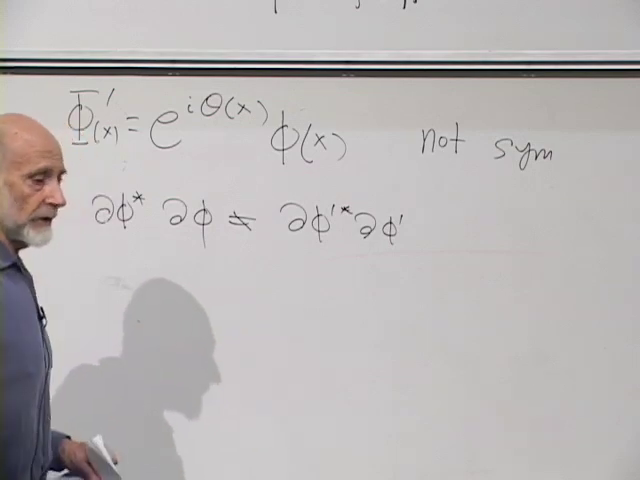
\includegraphics[width=0.78\textwidth]{lecture_08_figure_04.png}
\caption{Die Tafel hält die lokale Phasentransformation und das Versagen des gewöhnlichen Ableitungsterms, invariant zu bleiben, fest.}
\lectureframe{00:46:49}
\label{fig:l08-local-not-symmetry}
\end{figure}

Wir führen ein Vektorpotential ein und legen eine Konvention fest, die wir konsequent beibehalten:
\begin{equation}
  D_\mu=\partial_\mu+i g A_\mu,
  \qquad
  A_\mu'=A_\mu-\frac1g\partial_\mu\theta.
  \label{eq:l08-covariant-convention}
\end{equation}
Nun gilt
\begin{align}
  D_\mu'\phi'
  &=
  \left(\partial_\mu+i g A_\mu'\right)
  e^{i\theta}\phi
  \notag\\
  &=
  e^{i\theta}
  \left[
    \partial_\mu\phi+i(\partial_\mu\theta)\phi
    +i g A_\mu\phi-i(\partial_\mu\theta)\phi
  \right]
  \notag\\
  &=e^{i\theta}D_\mu\phi.
  \label{eq:l08-covariant-transform}
\end{align}
Die unerwünschten Terme heben sich auf. Die konjugierte Ableitung lautet
\begin{equation}
  (D_\mu\phi)^*
  =(\partial_\mu-i g A_\mu)\phi^*,
\end{equation}
und ihre entgegengesetzte Phase hebt sich im Produkt auf:
\begin{equation}
  (D_\mu\phi)^*D^\mu\phi.
\end{equation}

\begin{classroomqa}
\audiencequestion{War die Transformation des Eichfelds in der vorherigen Vorlesung mit umgekehrtem Vorzeichen angegeben?\lecturetimestamp{00:48:04}}
\lecturerresponse{Eine gleichzeitige Vorzeichenumkehr in \(D_\mu\) und im Transformationsgesetz ist lediglich eine Konvention. Bei \(D_\mu=\partial_\mu+i gA_\mu\) und \(\phi'=e^{i\theta}\phi\) muss für Konsistenz \(A_\mu'=A_\mu-g^{-1}\partial_\mu\theta\) gelten. Die alternative Konvention funktioniert ebenso gut, sofern alle Vorzeichen gemeinsam geändert werden.}
\end{classroomqa}

\begin{classroomqa}
\audiencequestion{Kennzeichnet die Verwendung einer Groß- oder Kleinbuchstabenform von \(\phi\) an der Tafel ein anderes Feld?\lecturetimestamp{00:55:02}}
\lecturerresponse{Nein, eine Unterscheidung ist nicht beabsichtigt. Die wechselnde Buchstabenform ist Handschrift, keine zusätzliche Operation und kein zweites Skalarfeld. Inhaltlich relevant sind der Strich, der Stern für die komplexe Konjugation und der Raumzeitindex.}
\end{classroomqa}

\begin{classroomqa}
\audiencequestion{Ist komplexe Konjugation dieselbe Operation wie das Heben oder Senken des Lorentz-Index im kinetischen Term?
\lecturetimestamp{00:56:50}}
\lecturerresponse{Nein. Der Stern komplex konjugiert das interne komplexe Feld. Lorentz-Indizes werden mit der Raumzeitmetrik gehoben:
\(D^\mu=g^{\mu\nu}D_\nu\). Ein Lorentz-Skalar erfordert die Kontraktion \((D_\mu\phi)^*D^\mu\phi\); beide Operationen kommen vor und erfüllen unterschiedliche Zwecke.}
\end{classroomqa}

\subsection{Das Eichfeld besitzt eine eigene Dynamik}

Der Feldstärketensor
\begin{equation}
  F_{\mu\nu}=\partial_\mu A_\nu-\partial_\nu A_\mu
  \label{eq:l08-field-strength}
\end{equation}
ist eichinvariant, weil sich die beiden gemischten zweiten Ableitungen von \(\theta\) aufheben. Seine Zeit--Raum-Komponenten enthalten das elektrische Feld, seine Raum--Raum-Komponenten das magnetische Feld. Die Elektrodynamik des Skalarfelds lautet daher
\begin{equation}
  \mathcal L
  =(D_\mu\phi)^*D^\mu\phi
  -V(\phi^*\phi)
  -\frac14F_{\mu\nu}F^{\mu\nu}.
  \label{eq:l08-abelian-higgs}
\end{equation}
Das geladene Feld ist hier bosonisch. Es ist nicht das Elektronenfeld, das ein Fermion ist. Ein geladener Heliumkern oder ein Cooper-Paar-Kondensat veranschaulicht, wie ein bosonischer geladener Freiheitsgrad entstehen kann.

Vor der Symmetriebrechung enthält der Eichterm Ableitungen von \(A_\mu\), aber keinen direkten Massenterm. Man könnte versuchen, \begin{equation}
  \frac12m_A^2A_\mu A^\mu,
\end{equation} hinzuzufügen, doch gemäß Gl. ~\eqref{eq:l08-covariant-convention} gilt
\begin{equation}
  A_\mu A^\mu
  \longmapsto
  \left(A_\mu-\frac1g\partial_\mu\theta\right)
  \left(A^\mu-\frac1g\partial^\mu\theta\right),
  \label{eq:l08-bare-mass-fails}
\end{equation}
was nicht gleich \(A_\mu A^\mu\) ist. Eine nackte Masse des Eichbosons ist durch die lokale Symmetrie verboten.

\begin{figure}[htbp]
\centering
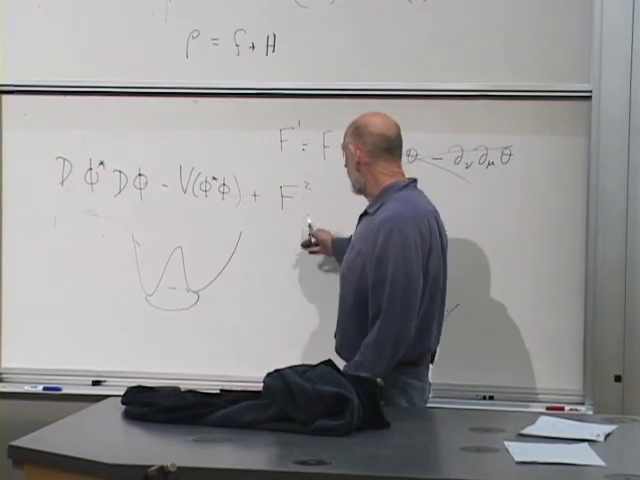
\includegraphics[width=0.76\textwidth]{lecture_08_figure_05.png}
\caption{Ein überprüfter Zustand der Tafel, der das Hindernis zeigt: Unter einer Eichtransformation wird \(A_\mu A^\mu\) zu einem Quadrat, das \(\partial_\mu\theta\) enthält; eine nackte Vektormasse ist daher nicht invariant.}
\lectureframe{01:07:30}
\label{fig:l08-bare-mass-board}
\end{figure}

\section{Der Higgs-Mechanismus}

\subsection{Die kovariante Ableitung erzeugt die Masse}

Wir kehren zum gebrochenen Potential zurück und verwenden die kanonisch normierte Parametrisierung
\begin{equation}
  \phi(x)=\frac{f+h(x)}{\sqrt2}
  e^{i\pi(x)/f}.
\end{equation}
Ihre kovariante Ableitung lautet
\begin{equation}
  D_\mu\phi
  =
  \frac{e^{i\pi/f}}{\sqrt2}
  \left[
    \partial_\mu h
    +i(f+h)
      \left(\frac{\partial_\mu\pi}{f}+gA_\mu\right)
  \right].
  \label{eq:l08-covariant-polar}
\end{equation}
Folglich gilt
\begin{equation}
\begin{aligned}
  (D_\mu\phi)^*D^\mu\phi
  ={}&
  \frac12(\partial_\mu h)^2
  \\
  &+\frac12(f+h)^2
    \left(\frac{\partial_\mu\pi}{f}+gA_\mu\right)
  \\
  &\hspace{4.2em}\times
    \left(\frac{\partial^\mu\pi}{f}+gA^\mu\right).
\end{aligned}
  \label{eq:l08-higgs-kinetic}
\end{equation}

Der entscheidende Term tritt bereits vor jeder Eichwahl auf:
\begin{equation}
  \frac12g^2f^2 A_\mu A^\mu.
  \label{eq:l08-vector-mass-term}
\end{equation}
Vergleichen wir ihn mit der Proca-Form \(\frac12m_A^2A_\mu A^\mu\), erhalten wir
\begin{equation}
  \boxed{m_A=g f}.
  \label{eq:l08-vector-mass}
\end{equation}
Dieselbe Entwicklung liefert auch die Wechselwirkungen \(g^2fh A_\mu A^\mu\) und \(\frac12g^2h^2A_\mu A^\mu\). Die Vektormasse ist also keine willkürliche Verletzung der Eichsymmetrie. Sie entsteht aus einem eichinvarianten kinetischen Skalarfeldterm, ausgewertet in einer Phase mit nicht verschwindendem Gleichgewichtsbetrag \(f\).

\begin{figure}[htbp]
\centering
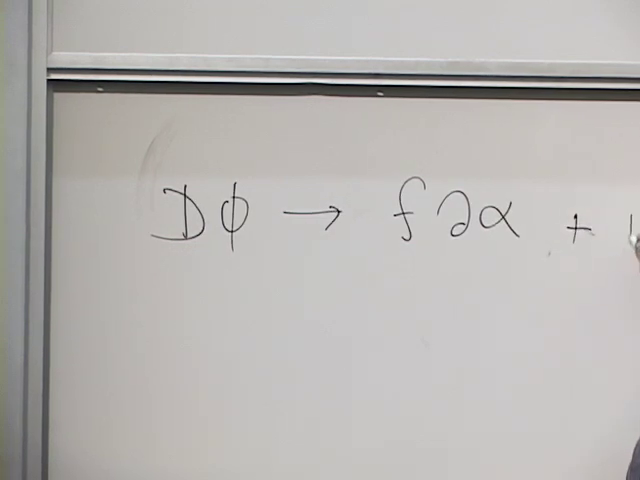
\includegraphics[width=0.78\textwidth]{lecture_08_figure_06.png}
\caption{Die Tafel isoliert den Beitrag \(f^2A^2\) innerhalb von \((D\phi)^*(D\phi)\). Numerische Faktoren hängen davon ab, wie das Skalarfeld und die Eichkopplung normiert sind; mit Gl. ~\eqref{eq:l08-canonical-polar} und \eqref{eq:l08-covariant-convention} ergibt sich \(m_A=gf\).}
\lectureframe{01:10:10}
\label{fig:l08-generated-mass-board}
\end{figure}

Die Vorlesung nimmt \(g\) und mehrere Faktoren von \(\sqrt2\) in ihre Tafelschreibweise auf. Daher wechselt sie bei der Bestimmung der Masse kurz zwischen \(f\), \(2f\) und \(\sqrt2f\). Diese Faktoren haben keine invariante Bedeutung, solange die Normierungen des kinetischen Terms und des Potentials nicht angegeben sind. Das robuste Ergebnis ist \(m_A\propto gf\); Gl. ~\eqref{eq:l08-vector-mass} gibt den Faktor für die hier verwendete Konvention an.

\subsection{Die Phase wird absorbiert}

Unter einer Eichtransformation ändert sich die Phasenvariable gemäß
\begin{equation}
  \pi'(x)=\pi(x)+f\,\theta(x).
\end{equation}
Wir wählen
\begin{equation}
  \theta(x)=-\frac{\pi(x)}{f}.
  \label{eq:l08-unitary-gauge-choice}
\end{equation}
Dann gilt \(\pi'=0\). Dies ist die unitäre Eichung, in der \begin{equation}
  \phi'(x)=\frac{f+h(x)}{\sqrt2}
\end{equation} reell ist, und Gl. ~\eqref{eq:l08-higgs-kinetic} vereinfacht sich zu
\begin{equation}
  (D_\mu\phi')^*D^\mu\phi'
  =
  \frac12(\partial_\mu h)^2
  +\frac12g^2(f+h)^2A_\mu'A^{\prime\mu}.
  \label{eq:l08-unitary-gauge-lagrangian}
\end{equation}
Das winkelabhängige Goldstone-Feld ist aus der Liste der unabhängigen Variablen verschwunden, während die Vektormasse erhalten bleibt.

Die Vorlesung zeigt dies zunächst im Grenzfall niedriger Energien \(\rho=f\), in dem
\begin{align}
  \phi&=f e^{i\alpha},
  \notag\\
  D_\mu\phi
  &=if e^{i\alpha}
    \left(\partial_\mu\alpha+gA_\mu\right),
  \notag\\
  (D_\mu\phi)^*
  &=-if e^{-i\alpha}
    \left(\partial_\mu\alpha+gA_\mu\right).
  \label{eq:l08-frozen-radius}
\end{align}
Ihr Produkt ist
\begin{equation}
  f^2
  \left(\partial_\mu\alpha+gA_\mu\right)
  \left(\partial^\mu\alpha+gA^\mu\right).
\end{equation}
Die Wahl \(\theta=-\alpha\) lässt \(g^2f^2A_\mu'A^{\prime\mu}\) übrig.

\begin{figure}[htbp]
\centering
\includegraphics[width=0.82\textwidth]{lecture_08_figure_07.png}
\caption{Der vollständige Tafelausdruck bei festgehaltenem Radius: Die kovarianten Ableitungen enthalten gemeinsam die Phasenableitung und das Vektorpotential. Als Nächstes wählt die Vorlesung \(\theta=-\alpha\), eliminiert dadurch die Phase und lässt den Vektormassenterm zurück.}
\lectureframe{01:16:20}
\label{fig:l08-frozen-radius-board}
\end{figure}

\begin{classroomqa}
\audiencequestion{Lässt sich die gesamte Lagrange-Funktion in Variablen umschreiben, die das Verschwinden des Winkelmodus explizit machen?
\lecturetimestamp{01:13:49}}
\lecturerresponse{Ja. In Polarkoordinaten tritt die Phase nur über die eichinvariante Kombination \(\partial_\mu\alpha+gA_\mu\) auf. Eine Eichtransformation mit \(\theta=-\alpha\) setzt die Phase überall dort auf null, wo diese Eichung wohldefiniert ist. Der kinetische Skalarfeldterm wird dann zu einem Vektormassenterm, während der eichinvariante Feldstärketerm unverändert bleibt.}
\end{classroomqa}

\begin{classroomqa}
\audiencequestion{Sind Schwingungen in \(\alpha\) nicht von Eichschwingungen zu unterscheiden?\lecturetimestamp{01:18:02}}
\lecturerresponse{In der geeichten Theorie ist eine reine Änderung von \(\alpha\), die durch die entsprechende Änderung von \(A_\mu\) kompensiert wird, eine Eich-Neubeschreibung und keine eigenständige physikalische Welle. Die invariante Größe ist \(\partial_\mu\alpha+gA_\mu\). Der physikalische Modus, der durch das globale Goldstone-Feld dargestellt wurde, tritt als longitudinale Polarisation des massiven Vektors wieder auf.}
\end{classroomqa}

Es ist üblich, von einer spontan gebrochenen lokalen Eichsymmetrie zu sprechen. Diese Ausdrucksweise ist in der Praxis nützlich: Nach einer Eichwahl hat das Skalarfeld einen von null verschiedenen Vakuumwert, und das Spektrum enthält einen massiven Vektor. Genau genommen verbinden Eichtransformationen jedoch redundante Beschreibungen und keine verschiedenen physikalischen Zustände.
\editorialnote{Eine lokale Eichredundanz ist nicht im selben eichinvarianten Sinn gebrochen wie eine globale Symmetrie. Präzise lautet die Aussage, dass sich die Theorie in einer Higgs-Phase befindet. Die eichfixierte Störungstheorie beschreibt diese Phase durch einen von null verschiedenen Erwartungswert des Skalarfelds und das daraus folgende Spektrum mit massivem Vektor.}

\section{Wohin der Goldstone-Freiheitsgrad ging}

Nichts Physikalisches kann allein dadurch verschwinden, dass wir die Variablen wechseln. Zählen wir die Freiheitsgrade vor und nach dem Übergang in die Higgs-Phase.

Vorher:
\begin{equation}
  \underbrace{2}_{\text{massless vector}}
  +
  \underbrace{2}_{\text{complex scalar}}
  =4.
\end{equation}
Ein masseloser Vektor hat zwei transversale Polarisationen. Das komplexe Skalarfeld hat zwei reelle Komponenten: eine radiale und eine winkelabhängige.

Nachher:
\begin{equation}
  \underbrace{3}_{\text{massive vector}}
  +
  \underbrace{1}_{\text{radial Higgs}}
  =4.
  \label{eq:l08-degree-count}
\end{equation}
Ein massiver Vektor lässt sich in sein Ruhesystem bringen. Dort ist keine räumliche Richtung ausgezeichnet, daher muss er drei Polarisationszustände besitzen. Bei Bewegung sind zwei davon transversal und einer longitudinal. Der Goldstone-Modus ist zu dieser longitudinalen Polarisation geworden.

\begin{figure}[htbp]
\centering
\begin{adjustbox}{max width=\linewidth}
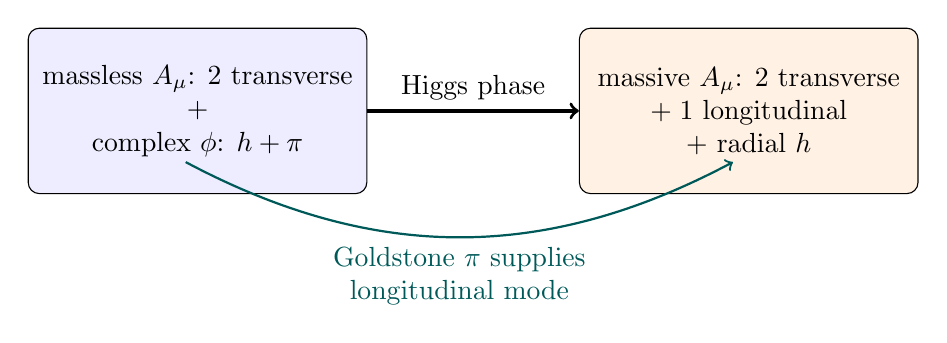
\begin{tikzpicture}[x=1cm,y=1cm]
  \node[draw,rounded corners,fill=blue!7,minimum width=4.3cm,
        minimum height=2.1cm,align=center] (before) at (0,0)
    {massless \(A_\mu\): \(2\) transverse\\
     \(+\)\\
     complex \(\phi\): \(h+\pi\)};
  \node[draw,rounded corners,fill=orange!10,minimum width=4.3cm,
        minimum height=2.1cm,align=center] (after) at (7,0)
    {massive \(A_\mu\): \(2\) transverse\\
     \(+\;1\) longitudinal\\
     \(+\) radial \(h\)};
  \draw[->,very thick] (before) -- node[above]{Higgs phase} (after);
  \draw[->,teal!70!black,thick]
    (-0.15,-0.65) to[bend right=28]
    node[below,align=center]{Goldstone \(\pi\) supplies\\longitudinal mode}
    (6.8,-0.65);
\end{tikzpicture}
\end{adjustbox}
\caption{Der Higgs-Mechanismus ordnet die physikalischen Freiheitsgrade neu, statt sie zu vernichten.}
\label{fig:l08-degree-rearrangement}
\end{figure}

\begin{classroomqa}
\audiencequestion{Wie kann der winkelabhängige Freiheitsgrad verschwinden, ohne die Zählung der Freiheitsgrade zu verletzen?\lecturetimestamp{01:19:13}}
\lecturerresponse{Physikalisch verschwindet er nicht. Ein masseloser Vektor hat zwei Helizitäten, weil er nicht in sein Ruhesystem gebracht werden kann. Ein massiver Vektor hat drei Polarisationen, darunter eine longitudinale. Der Goldstone-Modus wird zu dieser dritten Polarisation, sodass die Gesamtzahl unverändert bleibt.}
\end{classroomqa}

Die Vorlesung bietet einen nützlichen kinematischen Test. Man stelle sich ein massives Vektorteilchen vor, bremse es bis zum Stillstand ab und beschleunige es in eine neue Richtung. Eine Polarisation, die bezüglich der ursprünglichen Bewegungsrichtung transversal war, kann bezüglich der neuen Richtung longitudinal werden. Ebenso kehrt sich die Helizitätsbezeichnung um, wenn ein zirkular polarisiertes massives Teilchen durch den Ruhezustand gebracht und in die entgegengesetzte Richtung geschickt wird. Ein streng masseloses Teilchen kann dieses Experiment nicht durchlaufen, denn kein Inertialsystem kann es zum Stillstand bringen. Seine beiden Helizitäten bilden daher ein konsistentes physikalisches Spektrum.

\section{Das Analogon im Supraleiter}

In einem herkömmlichen Supraleiter bilden Elektronen Cooper-Paare. Ein Paar ist ein Boson mit elektrischer Ladung \(2e\), und das Kondensat wird durch einen geladenen komplexen Ordnungsparameter beschrieben. Ist sein Betrag ungleich null, erzeugt die Kombination aus seiner Phase und dem elektromagnetischen Vektorpotential den Anderson--Higgs-Mechanismus. Statische Magnetfelder klingen über die London-Eindringtiefe ab, statt sich frei durch das Volumen auszubreiten. In diesem präzisen, vom Medium abhängigen Sinn verhält sich das Photon, als hätte es Masse erhalten.

Dieses Beispiel verdeutlicht auch die anfängliche Unterscheidung. Das elektromagnetische Feld wird nicht dauerhaft in ein anderes Elementarteilchen umgewandelt. Das massive Ausbreitungsgesetz gilt für den kollektiven Zustand im Inneren des Materials; außerhalb bleibt das Photon im Vakuum masselos.

\section{Was gezeigt wurde}

Das Argument lässt sich nun zusammenfassen, ohne seine Logik zu verlieren:
\begin{enumerate}
  \item Eine gebrochene globale kontinuierliche Symmetrie besitzt eine flache Winkelrichtung und daher einen masselosen Goldstone-Modus.
  \item Lokale Phaseninvarianz erfordert ein Eichpotential und ersetzt \(\partial_\mu\) durch \(D_\mu\).
  \item Eine nackte Masse für \(A_\mu A^\mu\) verletzt das lokale Transformationsgesetz.
  \item Besitzt das geladene Skalarfeld einen von null verschiedenen Gleichgewichtsbetrag \(f\), enthält der eichinvariante Term \(|D_\mu\phi|^2\) den Beitrag \(\frac12g^2f^2A_\mu A^\mu\).
  \item Die Phase lässt sich durch eine Eichwahl entfernen, und ihr physikalischer Freiheitsgrad wird zur longitudinalen Polarisation des massiven Vektors.
  \item Die radiale Higgs-Anregung bleibt erhalten; ihre Masse wird durch die Krümmung des Skalarfeldpotentials festgelegt.
\end{enumerate}

Als Nächstes müssen wir Fermionen ihre Massen verleihen. Elektronen und Quarks können den Vektormechanismus nicht direkt nutzen; ihre Kopplungen an das Higgs-Feld sind Yukawa-Wechselwirkungen. Sobald sich das Skalarfeld bei \(f\) einpendelt, werden diese Wechselwirkungen zu Fermionmassentermen.

Die allgemeine Aussage, dass vertraute Teilchen ohne elektroschwache Symmetriebrechung masselos wären, bedarf noch einer letzten Einschränkung. Die Massen der elementaren Quarks und geladenen Leptonen sowie die Massen von \(W\) und \(Z\) verschwinden tatsächlich mit dem Higgs-Erwartungswert. Der größte Teil der Protonen- und Neutronenmasse entsteht jedoch dynamisch durch QCD-Confinement und die Energie des starken Feldes, nicht durch die Higgs-Massen der Quarks. Diese Unterscheidung ändert nichts am hier hergeleiteten Higgs-Mechanismus; sie grenzt seinen Anwendungsbereich präzise ab.
